\documentclass[12pt]{article}

\usepackage{tikz}
\usetikzlibrary{shapes}
\newcommand{\ceil}[1]{\left\lceil#1\right\rceil}
\newcommand{\floor}[1]{\left\lfloor#1\right\rfloor}
\begin{document}


\begin{figure}[h]
\centering
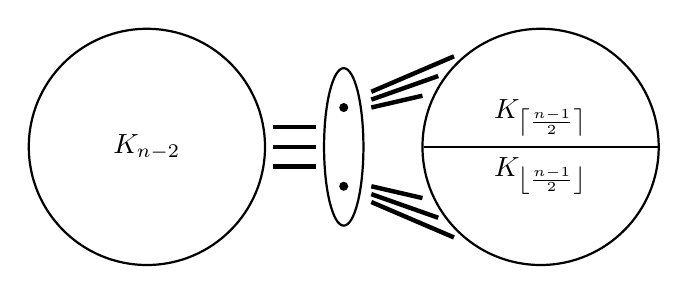
\begin{tikzpicture}[scale = 1]

\node[circle, minimum width=3cm, thick, draw] (L) at (0,0) {$K_{n-2}$};
\node[ellipse, minimum height=2cm, minimum width=0.5cm, thick, draw] (M) at (2.5,0) {};      
\node[circle split, minimum width=3cm, thick, draw] (R) at (5,0) 
{$K_{\ceil{\frac{n-1}{2}}}$ \nodepart{lower} $K_{\floor{\frac{n-1}{2}}}$};
\node[circle, inner sep =1pt, fill, draw] (P1) at (2.5,-0.5) {};
\node[circle, inner sep =1pt, fill, draw] (P2) at (2.5,0.5) {};

\draw (L) (M) (R) (P1) (P2);
\draw[ultra thick] (1.6,-.25) -- (2.15,-.25);
\draw[ultra thick] (1.6,0) -- (2.15,0);
\draw[ultra thick] (1.6,.25) -- (2.15,.25);

\draw[ultra thick] (2.85,-.7) -- (3.9,-1.15);
\draw[ultra thick] (2.85,-.6) -- (3.7,-.9);
\draw[ultra thick] (2.85,-.5) -- (3.5,-.65);

\draw[ultra thick] (2.85,.7) -- (3.9,1.15);
\draw[ultra thick] (2.85,.6) -- (3.7,.9);
\draw[ultra thick] (2.85,.5) -- (3.5,.65);
\end{tikzpicture}
\end{figure}

\end{document}
